%!TEX root = ../main.tex
\chapter{Krav}

I dette afsnit beskrives de opstillede krav for AVS. På \ref{photo:UseCD} ses det færdige Use Case diagram over systemet, dett et ligger til grund for de funktionelle krav.

\begin{figure}[H]
	\centering
	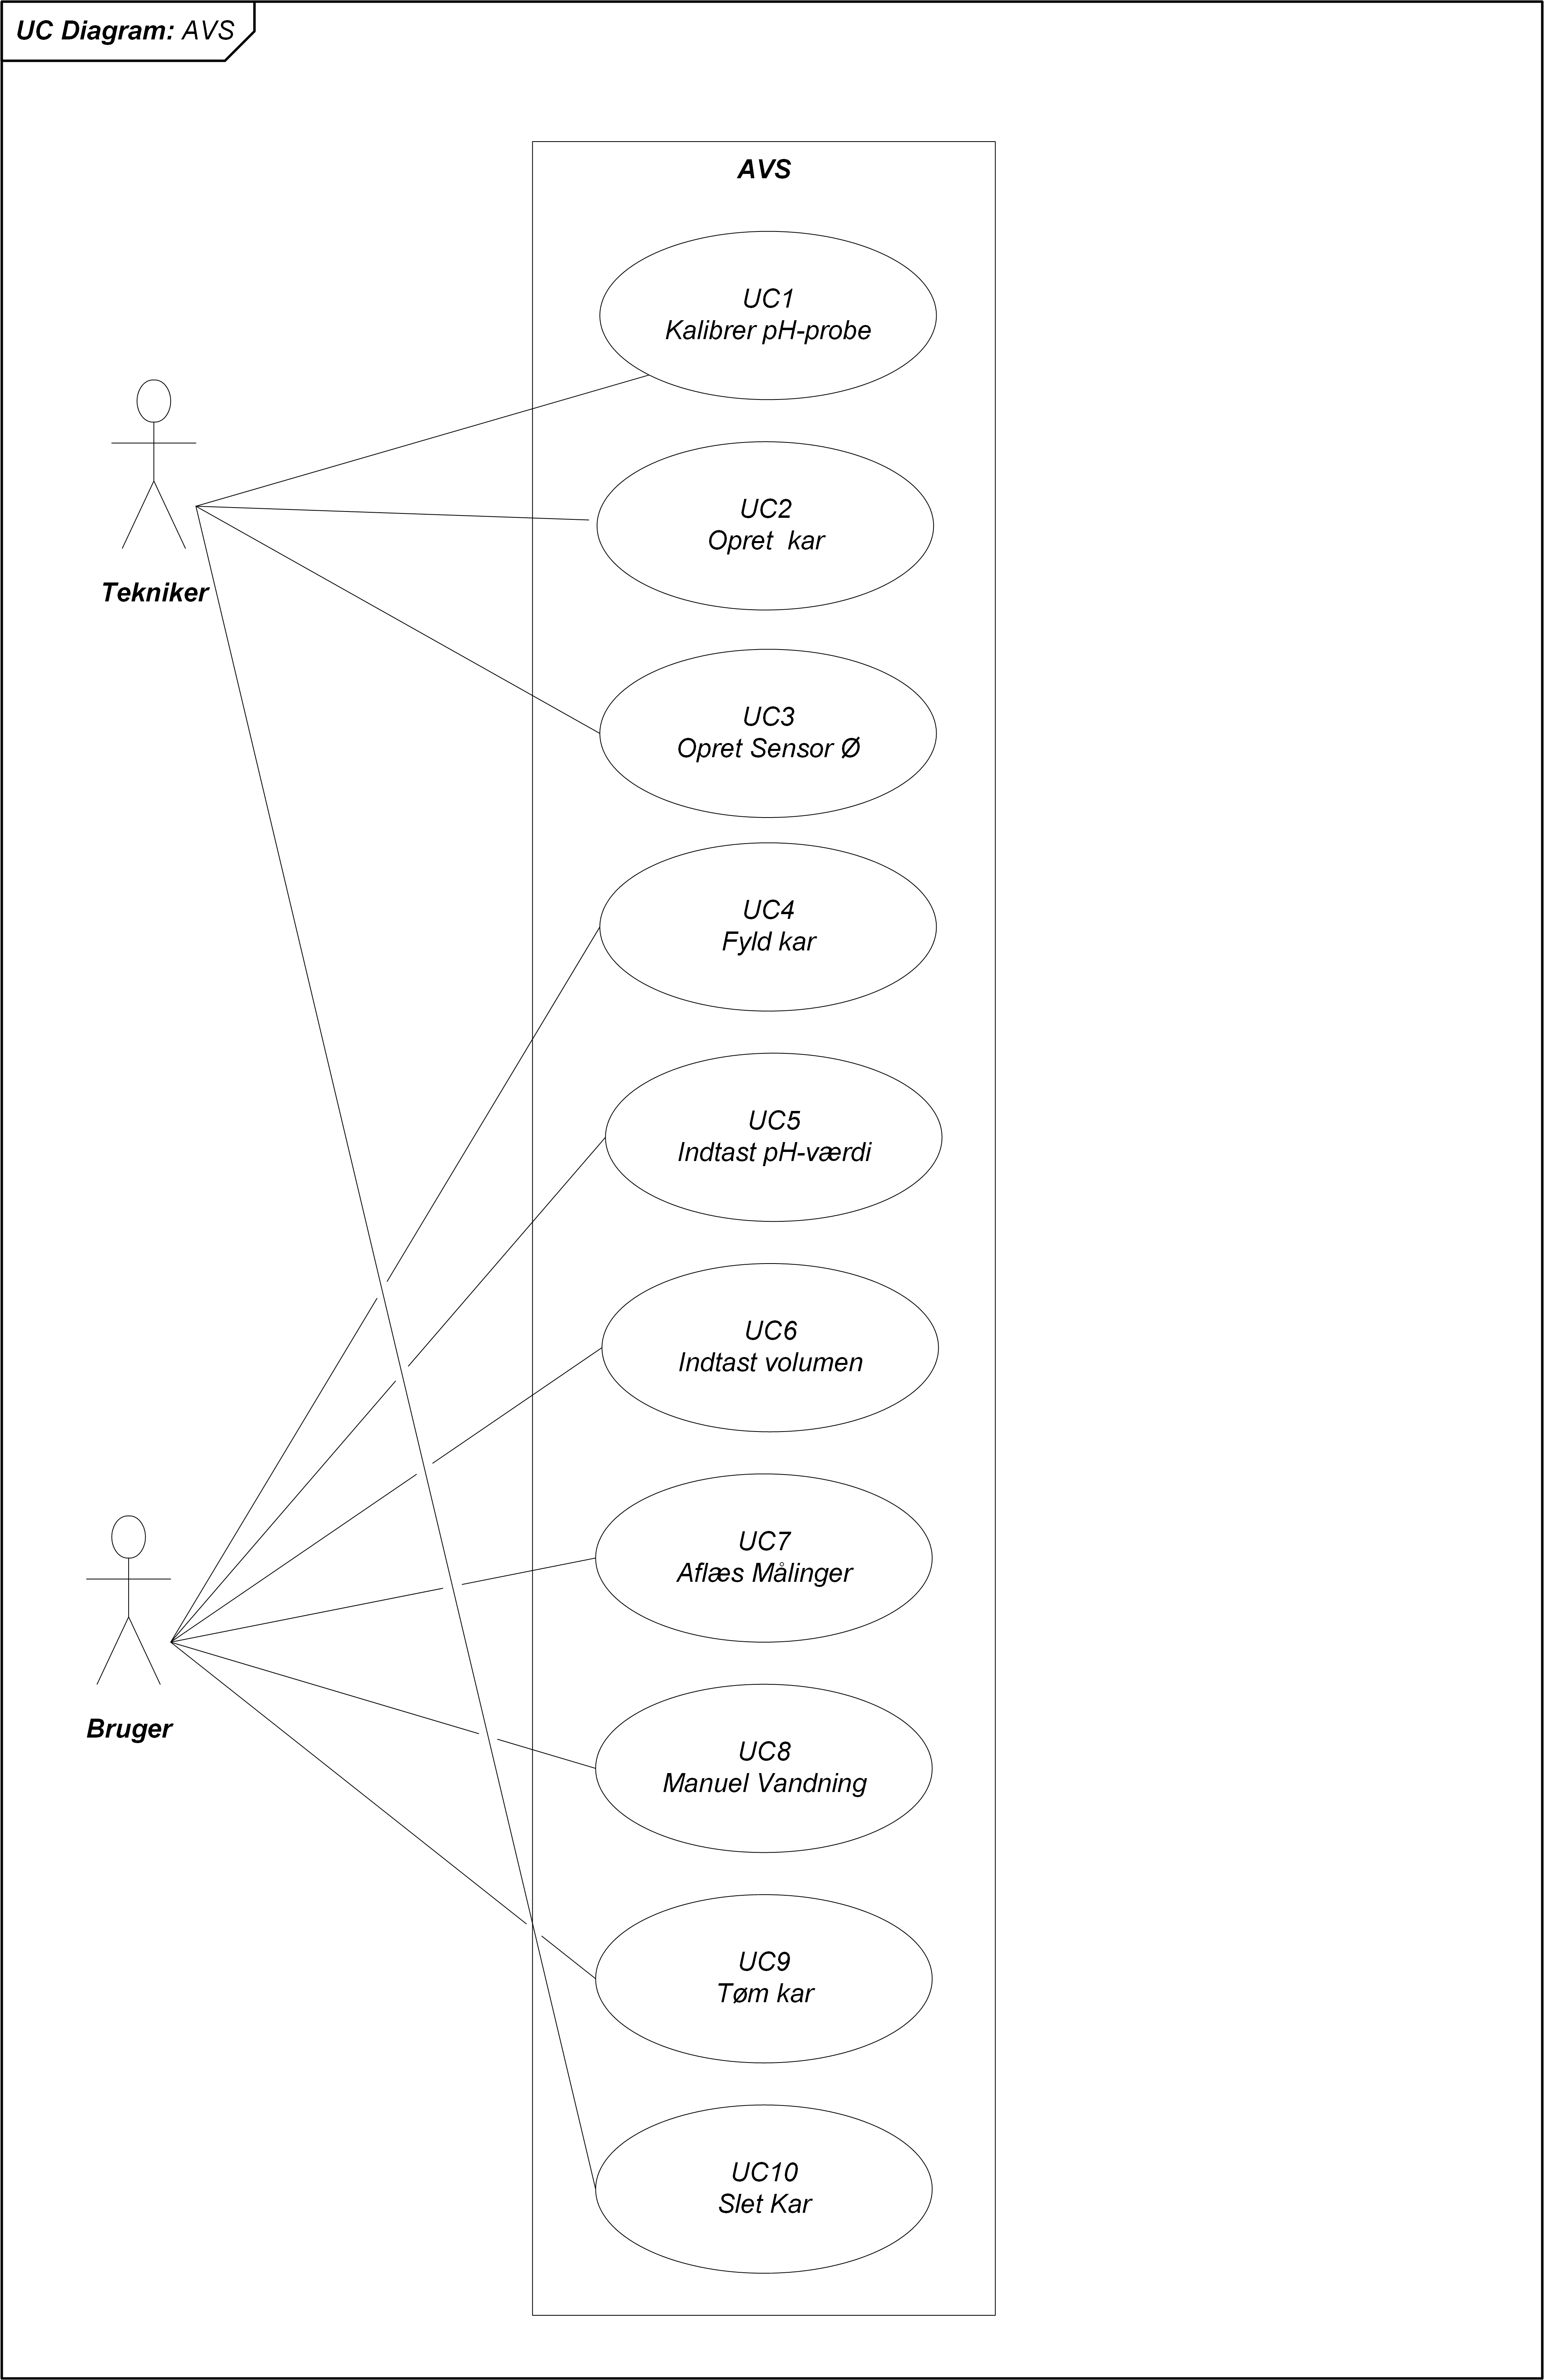
\includegraphics[scale=0.6]{Krav/Billeder/AVS_UseCases}
	\caption{AVS Use case diagram}
	\label{photo:UseCD}
\end{figure}

Herunder findes en kort beskrivelse af de enkelte use cases. For yderlige detaljer henvises til Projektdokumentationen under afsnit 1.2 "Use Cases"

\textbf{Use Case 1 - Kalibrer pH-Probe} \\
Denne use case har til formål at lade Teknikeren kalibrere den pH-probe der er tilsluttet et givent kar. Denne use case skal køres hver gang systemet startes op.\newline

\textbf{Use Case 2 - Opret kar} \\
Denne use case har til formål at lade Teknikeren oprette et nyt Kar til systemet, dette udføres fra Gui'en i brugerens webbrowser. \newline

\textbf{Use Case 3 - Opret Sensor Ø} \\
Denne use case har til formål at lade Teknikeren oprette en ny SensorØ til systemet, dette udføres fra Gui'en i brugerens web-browser.\newline

\textbf{Use Case 4 - Fyld kar} \\
Denne use case har til formål at lade Brugeren åbne for indløbsventilen og fylde karet med vand.\newline

\textbf{Use Case 5 - Indtast pH-værdi} \\
Denne use case har til formål at lade Brugeren indtaste en ønsket pH-værdi via Gui'en. Herefter justerer systemet Gødning/vand indtil den indtastede pH-værdi er opnået. \newline

\textbf{Use Case 6 - Indtast volumen} \\
Denne use case har til formål at lade Brugeren indtaste en ønsket volumen via Gui'en. Herefter justerer systemet ind- og afløbsventiler indtil den indtastede volumen er opnået.\newline

\textbf{Use Case 7 - Aflæs målinger} \\
Denne use case har til formål at lade Brugeren tilgå de tilkoblede kar via Gui'en og aflæse ønskede data.\newline

\textbf{Use Case 8 - Manuel vanding} \\
Denne use case har til formål at lade Brugeren, manuel tilføre vand til gromediet.\newline

\textbf{Use Case 9 - Tøm kar} \\
Denne use case har til formål at lade Brugeren åbne for afløbsventilen, tænde pumpen og tømme karet for vand.\newline

\textbf{Use Case 10 - Slet kar} \\
Denne use case har til formål at lade Teknikeren, via Gui'en slette et givent kar fra systemet.\newline


Derudover er følgende use cases tilføjet systemet, dog på ikke-fullydressed basis. For yderlige detaljer om de enkelte use cases refereres til Projektdokumentationen under afsnit 1.3 "Ikke fully dressed Use Cases"\\\

\textbf{Use Case 11 - Doser pH-væske}
Denne use case har til formål at Brugeren får mulighed for, manuelt at dosere pH-væske via en doseringspumpe indtil den
ønskede pH-værdi er opnået.\newline

\textbf{Use Case 12 - Automatisk vanding} 
Denne use case har til formål at lade vandingen ske automatisk, baseret på den målte jordfugtighed.\newline

\textbf{Use Case 13 - Alarm} 
Denne use case har til formål at lade Systemet afgive en alarm hvis de brugerdefineret grænseværdier (jordfugtighed, pH-værdi og volumen) overskrides.\newline

\textbf{Use Case 14 - Ugeplan} 
Denne use case giver Brugeren mulighed for at indtaste en ugeplan for styring af dosering af pH-væske
og vand til gromediet.\newline

\textbf{Use Case 15 - Udprint log} 
Denne use case giver Brugeren mulighed for at få udprintet en log over de hændelser der er forekommet i systemet, herunder optaget sensordata samt dosering af vand.\newline


For at sikre kvaliteten af det færdige produkt, er der opstillet en række krav. Disse er kort beskrevet herunder, for yderligere detaljer henvises til Projektdokumentationen under afsnit 1.4 "Ikke funktionelle krav"

Kravene er inddelt i 3 undergrupper: 

\begin{itemize}
	\item	Brugervenlighed
	\item	Systembetingelser
	\item	Ydelse
\end{itemize}

Kravene under brugervenlighed baserer sig på at systemet skal kunne kører på en "standard" PC og kunne tilgås igennem normal webbrowser. Derudover skal systemet kunne tilgås over lokalt netværk samt over www.\newline
Under Systembetingelser opsættes de miljømæssige omstændigheder under hvilke hvor systemet skal kunne opererer.\newline 
Ydelse opsætter de tider og grænseværdier for fyldning og tømning af systemet, samt for dosering af gødning og vand til gromediet.